%%=====================================================================================
%%
%%       Filename:  solution_6.tex
%%
%%    Description:  Solution to Assignment 6.
%%
%%        Version:  1.0
%%        Created:  03/26/2017
%%       Revision:  none
%%
%%         Author:  Dilawar Singh (), dilawars@ncbs.res.in
%%   Organization:  NCBS Bangalore
%%      Copyright:  Copyright (c) 2017, Dilawar Singh
%%
%%          Notes:  
%%                
%%=====================================================================================

\documentclass[a4paper,10pt]{article}
\usepackage{pgf,tikz}
\usepackage{amsmath}
\usepackage{pgfplots}
\usepackage[american]{circuitikz}
\usepackage{amssymb}
\usetikzlibrary{shapes,backgrounds,decorations,decorations.pathmorphing}
\usepackage{siunitx}
% Title Page
\title{Solution to problem 6} 
\author{Dilawar Singh}
\date{\today}

\begin{document}
\maketitle

\paragraph{Problem A, 9 points}

I change the extracellular solution on a squid axon so it has 50 mM K+ ions. 

\begin{enumerate}
    \item What is the new reversal potential of the K channel?  
    \item Assume that the previous resting potential of \SI{-65}{\milli\volt} was 
        due to a leak at \SI{0}{\milli \volt} through $R_m$, in parallel with the 
        previous reversal potential of the K channel of about 
        \SI{-75}{\milli \volt}. What is the ratio of $R_m$ to the resting 
        conductance of the K channel?
    \item What is the new resting potential ($V_m$) of the cell, assuming that 
        the conductance of the K channel and Rm are still in the same ratio?
\end{enumerate}

\paragraph{Solution} 

\paragraph{Solution 1} \SI{-50}{\milli \volt}. See the figure \ref{fig:problema}

\begin{figure}[ht!]
\begin{center}
\begin{tikzpicture}[scale=1]
    \begin{axis}[ xlabel=$K^+$,ylabel=Equilibrium Potential (V)
            , grid style={draw=gray!20}, grid = both 
        ]

        \edef\Function{(8.314*279.3)/(9.648e4)*log(x/400)};
        \addplot [color=blue] gnuplot [ raw gnuplot ] {
                f(x)=\Function;
                plot [10:100] f(x) with linespoints;
            };

        \addplot+ [nodes near coords,only marks,mark=*] gnuplot [ raw gnuplot ] {
                f(x)=\Function;
                set samples 5;
                plot [10:90] f(x);
            };
        
    \end{axis}
\end{tikzpicture}
\end{center}
\caption{At $[K^+] =\SI{50}{\milli M}$, the value of potassium channel
equilibrium potential is \SI{-50}{\milli \volt} }
\label{fig:problema}
\end{figure}

Following is the equivalent circuit for this problem. We expect the cell resting
potential to be \SI{-65}{\milli \volt}. 

$$ \frac{-65}{R_m}  + \frac{-65 +75}{R_K} = 0$$
$$ R_m = 6.5 R_K $$

\begin{tikzpicture}[scale=1 , every node/.style={} ]
    \draw[-*] (0,0) -- (1,0) node[above] {$-65 mV$};
    \draw (0,0) to[R=$R_m$] (0,-2) to[V=$0 V$] (0,-4);
    \draw (2,0) to[R=$R_K$] (2,-2) to[V=$-75 V$] (2,-4);
    \draw (0,0) -- (2,0);
    \draw (0,-4) -- (2,-4);
    \node[scale=3] at (1,-2)  {$\circlearrowright$};
    \node[] at (1,-2)  {$i$};
\end{tikzpicture}    

To equivalent circuit for this problem is the following. We solve this circuit:

$$ i = \frac{-50}{R_m + R_K} $$
$$ V_m = i * R_m = \frac{-50 R_m}{R_m + R_K} = \frac{-50}{1 + \frac{R_K}{R_m}} =
\frac{-50}{1+0.1538} = - 43.335 $$


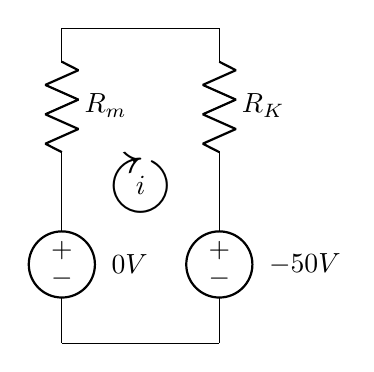
\begin{tikzpicture}[scale=1 , every node/.style={} ]
    %\draw[-*] (0,0) -- (1,0) node[above] {$-65 mV$};
    \draw (0,0) to[R=$R_m$] (0,-2) to[V=$0 V$] (0,-4);
    \draw (2,0) to[R=$R_K$] (2,-2) to[V=$-50 V$] (2,-4);
    \draw (0,0) -- (2,0);
    \draw (0,-4) -- (2,-4);
    \node[scale=3] at (1,-2)  {$\circlearrowright$};
    \node[] at (1,-2)  {$i$};
\end{tikzpicture}    



\paragraph{Problem B, 5 Points} The idea of ‘Dendritic Democracy’ states that a
neuron will experience the same depolarization at the cell body, regardless of
where the input comes in on a big dendritic arbor. Knowing what you do now of
dendritic signal propagation, receptors, and HH channels, suggest 3 ways in
which the cell could achieve dendritic democracy. In each case put in some
numbers indicating specific biophysical changes that the cell should undergo to
achieve this. Assume the cell is 2 lambda in electrotonic length.

\paragraph{Solution} Since membrane passive property does not change within a
neuron, the only way to achieve this if a synaptic input causes larger response
at far away site than to the proximal site. This way even when the signal
travels more distance from the distal site, its influence on soma will be
similar to the effect of signal from proximal site.

\begin{itemize}
    \item More receptors at the distal site compared to proximal site.
    \item Properties of HH Channels are different, higher $g_Na$ or lower $g_K$ (due
        to?) at distal site.
    \item The number of vesicle releases at distal site are more or the number
        of transmitters in per vesicle are more. Although its hard to say why
        this should be case at pre-synaptic site.
\end{itemize}

Lets see what you have written!


\paragraph{Problem C, 5 Points} A cell is full of voltage-gated ion channels, so
it undergoes back-propagating action potentials into its dendrites. When will a
synaptic input have more effect on the cell output: before, during or after the
action potential at the soma? Explain with one line each.


\paragraph{Problem D, 5 Points} What ion channels should a cell have to be of
type I (continuous frequency-current curve ) vs type II (having an abrupt
threshold at which it suddenly starts firing) ?

\end{document}          
